% ============================================================================
%  ADVANCED DATA STRUCTURES ACADEMIC STUDENT NOTES
%  UNIT 5: Pattern Matching Algorithms
% ============================================================================

\documentclass[11pt,a4paper]{article}

% ── Fonts ───────────────────────────────────────────────────────────────────
\usepackage[T1]{fontenc}
\usepackage{noto}

% ── Page Layout ─────────────────────────────────────────────────────────────
\usepackage[
  a4paper,
  left=1in,
  right=1in,
  top=1.15in,
  bottom=1.15in,
  headheight=22pt
]{geometry}

% ── Colors ──────────────────────────────────────────────────────────────────
\usepackage[dvipsnames,svgnames,table]{xcolor}

\definecolor{TheoremBlue}{RGB}{0,82,155}
\definecolor{DefinitionGreen}{RGB}{0,112,74}
\definecolor{ExampleOrange}{RGB}{184,84,0}
\definecolor{RemarkPurple}{RGB}{108,52,131}
\definecolor{NoteRed}{RGB}{179,0,0}
\definecolor{ChapterBlue}{RGB}{20,60,120}

% ── Math Packages ───────────────────────────────────────────────────────────
\usepackage{amsmath,amssymb,amsthm,mathtools}
\usepackage{mathrsfs}
\usepackage{bbm}

% ── Theorem Environments (tcolorbox) ────────────────────────────────────────
\usepackage[most]{tcolorbox}
\tcbuselibrary{theorems, skins, breakable}

\newtcbtheorem[number within=section]{theorem}{Theorem}{%
  enhanced,
  colback=TheoremBlue!4,
  colframe=TheoremBlue!80!black,
  coltitle=white,
  fonttitle=\bfseries,
  sharp corners,
  boxrule=0.8pt,
  top=6pt, bottom=6pt, left=8pt, right=8pt,
  separator sign none,
  description delimiters parenthesis,
  breakable
}{thm}

\newtcbtheorem[number within=section]{definition}{Definition}{%
  enhanced,
  colback=DefinitionGreen!4,
  colframe=DefinitionGreen!70!black,
  coltitle=white,
  fonttitle=\bfseries,
  rounded corners,
  boxrule=0.8pt,
  top=6pt, bottom=6pt, left=8pt, right=8pt,
  separator sign none,
  description delimiters parenthesis,
  breakable
}{def}

\newtcbtheorem[number within=section]{example}{Example}{%
  enhanced,
  colback=ExampleOrange!4,
  colframe=ExampleOrange!60!black,
  fonttitle=\bfseries,
  rounded corners,
  boxrule=0.6pt,
  borderline west={3pt}{0pt}{ExampleOrange!80},
  top=5pt, bottom=5pt, left=10pt, right=8pt,
  separator sign none,
  breakable
}{ex}

\newtcolorbox{remark}[1][]{%
  enhanced,
  colback=RemarkPurple!3,
  colframe=RemarkPurple!3,
  borderline west={2.5pt}{0pt}{RemarkPurple!70},
  sharp corners,
  boxrule=0pt,
  top=5pt, bottom=5pt, left=8pt, right=8pt,
  fontupper=\small,
  before upper={\textbf{\color{RemarkPurple}Remark.}\quad},
  breakable,
  #1
}

\newtcolorbox{notebox}[1][]{%
  enhanced,
  colback=NoteRed!3,
  colframe=NoteRed!3,
  borderline west={2.5pt}{0pt}{NoteRed!70},
  sharp corners,
  boxrule=0pt,
  top=5pt, bottom=5pt, left=8pt, right=8pt,
  before upper={\textbf{\color{NoteRed}Note.}\quad},
  breakable,
  #1
}

% ── TikZ Diagrams ───────────────────────────────────────────────────────────
\usepackage{tikz}
\usetikzlibrary{positioning, arrows.meta, shapes.geometric, calc, fit, backgrounds}

% ── Lists ───────────────────────────────────────────────────────────────────
\usepackage[shortlabels]{enumitem}
\setlist[enumerate]{topsep=4pt, itemsep=2pt, parsep=2pt}
\setlist[itemize]{topsep=4pt, itemsep=2pt, parsep=2pt}
\setlist[enumerate,1]{label=\arabic*.}

% ── Tables ──────────────────────────────────────────────────────────────────
\usepackage{booktabs}
\usepackage{array}
\usepackage{tabularx}

% ── Headers and Footers ────────────────────────────────────────────────────
\usepackage{fancyhdr}
\pagestyle{fancy}
\fancyhf{}
\fancyhead[L]{\color{gray}\small UNIT 5: Pattern Matching}
\fancyhead[R]{\color{gray}\small Advanced Data Structures}
\fancyfoot[C]{\thepage}
\renewcommand{\headrulewidth}{0.4pt}
\renewcommand{\footrulewidth}{0pt}

% ── Section Styling ─────────────────────────────────────────────────────────
\usepackage{titlesec}
\titleformat{\section}
  {\Large\bfseries\color{ChapterBlue}}
  {\thesection}{0.8em}{}

\titleformat{\subsection}
  {\large\bfseries\color{DefinitionGreen!80!black}}
  {\thesubsection}{0.8em}{}

% ── Hyperlinks & Cross-references ───────────────────────────────────────────
\usepackage[colorlinks=true, linkcolor=TheoremBlue, citecolor=TheoremBlue, urlcolor=TheoremBlue]{hyperref}
\usepackage[nameinlink,capitalize]{cleveref}

% ============================================================================
%  DOCUMENT BEGINS
% ============================================================================
\begin{document}

\begin{titlepage}
  \centering
  \vspace*{1.5cm}

  {\color{ChapterBlue}\rule{\textwidth}{1.5pt}}
  \vspace{0.6cm}
  {\fontsize{26}{32}\selectfont\bfseries\color{ChapterBlue} Advanced Data Structures}
  \vspace{0.4cm}
  {\Large\color{gray} Academic Student Notes}
  \vspace{0.4cm}
  {\color{ChapterBlue}\rule{\textwidth}{1.5pt}}

  \vspace{1.5cm}
  {\large\textbf{UNIT - V: Pattern Matching Algorithms}}

  \vspace{2cm}

  \begin{center}
    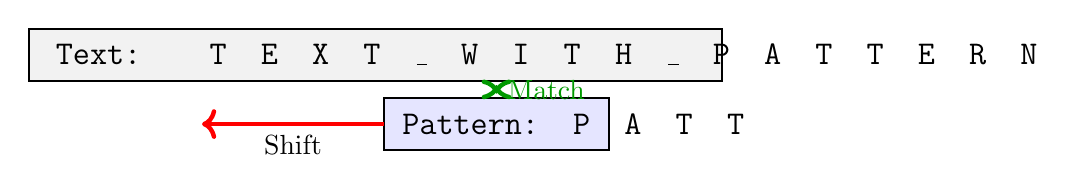
\begin{tikzpicture}[scale=1.1]
      % Graphic illustrating Text vs Pattern
      \draw[thick, fill=gray!10] (0, 0.8) rectangle (8, 1.4);
      \node[anchor=west] at (0.2, 1.1) {\large\texttt{Text: \ \ T \ E \ X \ T \ \_ \ W \ I \ T \ H \ \_ \ P \ A \ T \ T \ E \ R \ N}};

      \draw[thick, fill=blue!10] (4.1, 0) rectangle (6.7, 0.6);
      \node[anchor=west] at (4.2, 0.3) {\large\texttt{Pattern: P \ A \ T \ T}};

      \draw[red, ultra thick, ->] (4.1, 0.3) -- (2.0, 0.3) node[midway, below, text=black] {Shift};
      \draw[green!60!black, ultra thick, <->] (5.4, 0.65) -- (5.4, 0.75) node[midway, right] {Match};
    \end{tikzpicture}
  \end{center}

  \vspace{2cm}
  {\large\textit{Department of Computer Science and Engineering}} \\
  \vspace{0.2cm}
  {\large\textbf{Marri Laxman Reddy Institute of Technology and Management}} \\
  \vspace{0.1cm}
  {\small (UGC Autonomous, R25 Regulation)}

  \vfill
  {\normalsize Compiled: \today}
\end{titlepage}

\tableofcontents
\newpage

% ============================================================================
\section{Introduction to Pattern Matching}
% ============================================================================

The Pattern Matching problem is a fundamental challenge in computer science: given a large string of text $T$ of length $n$, and a pattern string $P$ of length $m$ (where $m \le n$), find one or all occurrences of $P$ inside $T$.

\begin{definition}{Terminologies}{terms}
  \begin{itemize}
    \item \textbf{Text ($T$)}: The main body of text to search within. Length is denoted as $n$.
    \item \textbf{Pattern ($P$)}: The substring we want to find. Length is denoted as $m$.
    \item \textbf{Shift ($s$)}: The alignment offset of the pattern relative to the text. We check if $T[s \dots s+m-1] = P[0 \dots m-1]$.
  \end{itemize}
\end{definition}

% ============================================================================
\section{Naive / Brute Force String Matching}
% ============================================================================

The \textbf{Brute Force} (or Naive) algorithm checks for a pattern match at all possible shift values from $s = 0$ up to $s = n - m$. At each shift, it compares character-by-character from left to right.

\begin{notebox}
  \textbf{Analogy}:
  Imagine trying to open a combination padlock by testing every single numeric combination starting from 000, 001, 002, and so on. If a digit doesn't work, you clear it, move to the next combination, and start testing digits from the first position again.
\end{notebox}

\subsection{Algorithm Mechanics}
For each shift $s$:
\begin{enumerate}
  \item Align the pattern $P$ at $T[s]$.
  \item Compare character $P[j]$ with $T[s+j]$ starting from $j = 0$.
  \item If all characters match ($j = m$), report a match at shift $s$.
  \item If a mismatch occurs at any $j$, increment shift to $s+1$, reset $j = 0$, and repeat.
\end{enumerate}

\subsection{Complexity Analysis}
\begin{itemize}
  \item \textbf{Worst-Case Complexity}: $O(m \cdot (n - m + 1))$. If $n \gg m$, this is $O(m \cdot n)$. This occurs when there are many partial matches (e.g., $T = \text{AAAAAAAAAAB}$ and $P = \text{AAAB}$).
  \item \textbf{Best-Case Complexity}: $O(n)$. Occurs when the first character of the pattern mismatch immediately (e.g., $T = \text{BBBBBBBBB}$ and $P = \text{AAA}$).
\end{itemize}

% ============================================================================
\section{Knuth-Morris-Pratt (KMP) Algorithm}
% ============================================================================

The \textbf{Knuth-Morris-Pratt} (KMP) algorithm improves execution speed by never backtracking in the text $T$. When a mismatch occurs, KMP uses precomputed information about the pattern itself to skip redundant alignments.

\begin{notebox}
  \textbf{Analogy}:
  Imagine reading a text and searching for the word \texttt{CHARACTER}. If you match \texttt{CHARAC} but mismatch at the next letter \texttt{T}, you don't go back in the text to read the second letter \texttt{H} again. You know you've already matched \texttt{CHARAC}, so you can safely shift forward past the matched prefix.
\end{notebox}

\subsection{The Prefix Function (Pi Table / Failure Function)}
The core of KMP is the $\pi$ table of length $m$. For each index $i$ in the pattern, $\pi[i]$ stores the length of the longest proper prefix of $P[0 \dots i]$ that is also a suffix of $P[0 \dots i]$.

\begin{example}{Computing the $\pi$ Table}{pi_table}
  Let's compute the $\pi$ table for the pattern $P = \text{ABABC}$:
  \begin{center}
    \textbf{Table 5.1: Prefix Function $\pi$ Table for $P = \text{ABABC}$} \\[0.5em]
    \begin{tabular}{cccccc}
      \toprule
      $i$      & 0 & 1 & 2 & 3 & 4 \\ \midrule
      $P[i]$   & A & B & A & B & C \\
      $\pi[i]$ & 0 & 0 & 1 & 2 & 0 \\ \bottomrule
    \end{tabular}
  \end{center}
  \begin{itemize}
    \item $\pi[0] = 0$: Substring "A" has no proper prefix.
    \item $\pi[1] = 0$: Substring "AB" has prefixes \{"A"\}, suffixes \{"B"\}. No match.
    \item $\pi[2] = 1$: Substring "ABA" has prefixes \{"A", "AB"\}, suffixes \{"A", "BA"\}. "A" matches (length 1).
    \item $\pi[3] = 2$: Substring "ABAB" has prefix "AB" which matches suffix "AB" (length 2).
    \item $\pi[4] = 0$: Substring "ABABC" has no prefix matching suffix because of "C".
  \end{itemize}
\end{example}

\subsection{KMP Search Execution}
When matching $T[i]$ against $P[j]$:
\begin{itemize}
  \item If $T[i] == P[j]$, increment both $i$ and $j$.
  \item If $j == m$, a match is found. Shift using $j = \pi[j-1]$.
  \item If $T[i] \neq P[j]$:
  \begin{itemize}
    \item If $j \neq 0$, do not decrement $i$. Instead, update $j = \pi[j-1]$ and check again.
    \item If $j == 0$, increment $i$ by 1.
  \end{itemize}
\end{itemize}

\subsection{Complexity Analysis}
\begin{itemize}
  \item \textbf{Preprocessing time}: $O(m)$ to build the $\pi$ table.
  \item \textbf{Matching time}: $O(n)$ because the index $i$ in the text never decreases.
  \item \textbf{Total Complexity}: $O(n + m)$.
\end{itemize}

\newpage

% ============================================================================
\section{Boyer-Moore Algorithm}
% ============================================================================

The \textbf{Boyer-Moore} (BM) algorithm is the gold standard for text search in text editors and command-line utilities (like grep). It compares characters from \textbf{right to left} (starting at the end of the pattern) but shifts the pattern from left to right.

\begin{notebox}
  \textbf{Analogy}:
  Imagine looking for a word in a word search puzzle. Instead of starting at the first letter, you look at the last letter. If that letter isn't even in the word you are looking for, you can jump the entire width of the word forward, saving a massive amount of scanning time.
\end{notebox}

Boyer-Moore uses two independent heuristics to determine how far it can shift the pattern on a mismatch:

\subsection{The Bad Character Heuristic}
When a mismatch occurs at $T[i] = c$ and $P[j] \neq c$:
1. If $c$ is not in the pattern $P$, shift the pattern completely past $T[i]$.
2. If $c$ is in the pattern $P$, shift the pattern to align the rightmost occurrence of $c$ in $P$ with $T[i]$.

Let $\text{last}[c]$ be the rightmost index of character $c$ in the pattern ($0$-indexed). If $c$ does not exist in $P$, $\text{last}[c] = -1$.
The shift distance is:
\begin{equation}
  \text{Shift} = j - \text{last}[c]
\end{equation}

\subsection{The Good Suffix Heuristic}
If a mismatch occurs after matching a suffix $t$ of the pattern:
1. Shift the pattern to align the matched suffix $t$ with its next rightmost occurrence in $P$.
2. If $t$ does not occur elsewhere, align a prefix of $P$ that matches a suffix of $t$ with $T$.
3. If no such overlap exists, shift the pattern completely past $t$.

\subsection{Shift Selection}
At each mismatch, Boyer-Moore calculates shifts from \textbf{both} the Bad Character rule and the Good Suffix rule, and shifts the pattern by the \textbf{maximum} of the two values.
\begin{itemize}
  \item \textbf{Worst-Case Complexity}: $O(m \cdot n)$ (occurs with repetitive text).
  \item \textbf{Best-Case Complexity}: $O(n / m)$ (sub-linear speed! We skip the majority of characters).
\end{itemize}

% ============================================================================
\section{Horspool's Algorithm}
% ============================================================================

\textbf{Horspool's Algorithm} is a simplified version of the Boyer-Moore algorithm. It retains the right-to-left comparison but uses \textbf{only} the Bad Character rule. It is highly efficient and simpler to implement.

Instead of looking at the mismatched character in $T$, Horspool's always determines the shift based on the character in the text aligned with the \textbf{last character} of the pattern, regardless of where the mismatch occurred.

\subsection{The Shift Table Calculation}
Let $\Sigma$ be the alphabet. For each character $c \in \Sigma$, the shift table value $d(c)$ is:
\begin{equation}
  d(c) = \begin{cases}
    m - 1 - i & \text{where } i \text{ is the rightmost index of } c \text{ in } P[0 \dots m-2] \\
    m         & \text{if } c \text{ is not in } P[0 \dots m-2]
  \end{cases}
\end{equation}

\begin{example}{Horspool Shift Table}{horspool}
  Let's compute the shift table for pattern $P = \text{BARBER}$ (length $m = 6$):
  \begin{itemize}
    \item Check characters in $P[0 \dots 4] = \text{BARBE}$.
    \item $d(\text{E}) = 6 - 1 - 4 = 1$
    \item $d(\text{B}) = 6 - 1 - 3 = 2$ (based on the second B at index 3)
    \item $d(\text{R}) = 6 - 1 - 2 = 3$
    \item $d(\text{A}) = 6 - 1 - 1 = 4$
    \item For any other character (like \text{R} at the end, or \text{X}), $d(c) = 6$.
  \end{itemize}
\end{example}

\subsection{Complexity Analysis}
\begin{itemize}
  \item \textbf{Average Case}: $O(n)$
  \item \textbf{Worst Case}: $O(m \cdot n)$
\end{itemize}

% ============================================================================
\section{Rabin-Karp Algorithm}
% ============================================================================

The \textbf{Rabin-Karp} algorithm uses hashing to search for the pattern. It computes a hash value for the pattern and for each window of length $m$ in the text.

\begin{notebox}
  \textbf{Analogy}:
  Imagine trying to find a matching page in a folder of documents. Instead of reading every line on every page, you count the number of words on each page. If a page doesn't have the same number of words as your target, you skip it instantly. If it does match, you do a detailed reading to confirm it is the correct page.
\end{notebox}

\subsection{Rolling Hash Function}
To make hashing fast, Rabin-Karp uses a \textbf{rolling hash}. The hash of the next window is calculated from the previous window in $O(1)$ time by subtracting the leading character and adding the trailing character.

Let $d$ be the size of the alphabet (radix), and $q$ be a prime number.
The hash value of $P[0 \dots m-1]$ is:
\begin{equation}
  p = (d^{m-1}P[0] + d^{m-2}P[1] + \dots + P[m-1]) \bmod q
\end{equation}
For a text window $T[s \dots s+m-1]$ with hash value $t_s$, the hash of the next window $t_{s+1}$ is:
\begin{equation}
  t_{s+1} = \left( d(t_s - T[s] \cdot h) + T[s+m] \right) \bmod q
\end{equation}
where $h = d^{m-1} \bmod q$.

\subsection{Handling Collisions}
If $p == t_s$, it is a potential match. Because different strings can produce the same hash value (a collision), the algorithm must verify character-by-character:
\begin{itemize}
  \item If they match exactly, report shift $s$.
  \item If not, it is a \textbf{spurious hit} (ignore and continue).
\end{itemize}

\subsection{Complexity Analysis}
\begin{itemize}
  \item \textbf{Best/Average Case}: $O(n + m)$ (if the hash function is good and causes few collisions).
  \item \textbf{Worst Case}: $O(m \cdot n)$ (occurs if the hash function is bad, causing collisions at every single step, requiring verification every time).
\end{itemize}

% ============================================================================
\section{Algorithm Comparison Summary}
% ============================================================================

\begin{table}[h]
  \centering
  \caption{Comparison of Pattern Matching Algorithms}
  \begin{tabularx}{\textwidth}{@{}lXXXX@{}}
    \toprule
    \textbf{Algorithm}  & \textbf{Preprocessing} & \textbf{Best Time} & \textbf{Worst Time} & \textbf{Space Complexity} \\ \midrule
    Naive / Brute Force & None                   & $O(n)$             & $O(m \cdot n)$      & $O(1)$                    \\
    KMP                 & $O(m)$                 & $O(n)$             & $O(n + m)$          & $O(m)$                    \\
    Boyer-Moore         & $O(m + |\Sigma|)$      & $O(n / m)$         & $O(m \cdot n)$      & $O(m + |\Sigma|)$         \\
    Horspool            & $O(m + |\Sigma|)$      & $O(n / m)$         & $O(m \cdot n)$      & $O(|\Sigma|)$             \\
    Rabin-Karp          & $O(m)$                 & $O(n + m)$         & $O(m \cdot n)$      & $O(1)$                    \\ \bottomrule
  \end{tabularx}
\end{table}

\end{document}
